\documentclass{article}
\usepackage{polski}
\usepackage{adjustbox}


\title{Dokumentacja systemu rejestrującego czas pracy}
\author{Wojciech Kozłowski}

\begin{document}
\maketitle
\section{Założenia symulacji}
Program jest napisany w języku python w wersji 3.6.
Program symuluje działanie czytnika kart RFID.
Projekt jest podzielony na podprogramy:
\begin{itemize}
    \item jeden program główny (będący serwerem)
    \item dowolna ilość programów symulujących termial z czytnikiem
        RFID.
\end{itemize}

\section{Implementacja}
\subsection{Serwer}
\subsubsection{Pola}

$\bullet$ \texttt{term\_file}, \texttt{logs\_file}, 
\texttt{card\_file} - nazwy plików w 
których składuje się dane (w formacie csv). \\
$\bullet$ \texttt{terminals} - lista zawierająca informacje o 
ID terminala i jego położeniu (\texttt{"in"} albo \texttt{"out"})\\
$\bullet$ \texttt{cards} - lista zawierająca informacje o 
numerze karty, imieniu i nazwisku jej posiadacza. \\
\subsubsection{Metody}
\hspace{0.13in}
$\bullet$ \texttt{load\_cards\_from\_file} - metoda pobierająca z pliku
o nazwie przechowywanej w \texttt{card\_file} identyfikatory
zarejestrowanych kart wzraz z imionami i nazwiskami ich posiadaczy.
Wszystkie informacje trafiają do pola \texttt{cards}. \\
\textbf{Argumenty} brak \\ \textbf{Zwraca} \texttt{None} \\

$\bullet$ \texttt{load\_term\_from\_file} - to samo co wyżej, ale 
informacje dotyczą terminali. \\
\textbf{Argumenty} brak \\ \textbf{Zwraca} \texttt{None} \\

\newpage 
$\bullet$ \texttt{append\_new\_card\_to\_file} - metoda 
dodająca informacje o nowo dodanej karcie do pliku. Metoda wykonywana
prywatnie, interface \texttt{Menu} nie pozwala się do niej dostać. \\
\textbf{Argumenty} brak \\ \textbf{Zwraca} \texttt{None} \\

$\bullet$ \texttt{append\_new\_term\_to\_file} - to samo dla 
terminali \\
\textbf{Argumenty} brak \\ \textbf{Zwraca} \texttt{None} \\

$\bullet$ \texttt{rewrite\_cards\_in\_file} - Po usunięciu, lub
modyfikacji danych związanych z kartami całość jest przepisywana na
nowo, ponieważ i tak przy zmianie w pliku trzeba byłoby przejść 
po każdej linii. Metoda wykonywana prywatnie. \\
\textbf{Argumenty} brak \\ \textbf{Zwraca} \texttt{None} \\

$\bullet$ \texttt{rewrite\_terms\_in\_file} - To samo dla terminali. \\
\textbf{Argumenty} brak \\ \textbf{Zwraca} \texttt{None} \\

$\bullet$ \texttt{add\_card} - dodaje nową karte do listy 
\texttt{cards}, oraz do pliku przechowującego informacje o kartach. 
Gdy karta z takim samym numerem już istnieje, to nie zostaje 
dodana.  \\
\textbf{Argumenty} \texttt{card\_num} - (str) numer karty (wartość,
która zostaje zwracana przez czytnik RFID), \texttt{username} - 
(str) imię właściciela (domyślnie puste), \texttt{usersurname} - 
(str) nazwisko właściciela (domyślnie puste). \\
\textbf{Zwraca} \texttt{None} \\

$\bullet$ \texttt{remove\_card} - karta o danym numerze zostaje
usunięta z danych serwera. \\
\textbf{Argumenty} \texttt{card\_num} - (int) numer karty 
do usunięcia \\ 
\textbf{Zwraca} \texttt{None} \\

$\bullet$ \texttt{add\_terminal} - dodaje nowy terminal o ile podane
ID nie istnieje w liście aktywnych terminali. \\
\textbf{Argumenty} \texttt{ID} - (str) ID terminalu,
\texttt{place} - (str) miejsce terminalu 
\texttt{"in"} lub \texttt{"out"} \\
\textbf{Zwraca} \texttt{None} \\

$\bullet$ \texttt{remove\_terminal} - dane o terminalu z podanym
ID zostaną usunięte z danych serwera. \\
\textbf{Argumenty} \texttt{terminalID} - (str) id terminala do 
usunięcia z danych. \\
\textbf{Zwraca} \texttt{None} \\

\newpage
$\bullet$ \texttt{find\_person} - zwraca imię i nazwisko osoby, 
która jest właścicielem karty o podanym numerze.\\
\textbf{Argumenty} \texttt{RFIDnum} - (int) numer karty RFID \\
\textbf{Zwraca} \texttt{None} \\

$\bullet$ \texttt{gate\_update} - dodaje akcje do logów.
Akcja to przejście właściciela karty o danym numerze przez 
bramke z danym terminalem.\\
\textbf{Argumenty} \texttt{ID} - (str) ID terminalu, który
wysłał informację, \texttt{RFIDnum} -
(str) numer karty, która została rozpoznana w terminalu.\\
\textbf{Zwraca} \texttt{None} \\

$\bullet$ \texttt{get\_logs} - zwraca liste list danych o wszystkich
przejsciach przez bramki.\\
\textbf{Argumenty} brak \\
\textbf{Zwraca} \texttt{list[list[str]]} \\

\subsection{Listener}
\subsubsection{Pola}

$\bullet$ \texttt{broker} - (str) adres IP (tutaj localhost) \\
$\bullet$ \texttt{client} - (mqtt.Client) obiekt, który odpowiada za
odbieranie wiadomości. \\
$\bullet$ \texttt{terget} - (Server) obiekt, na którym wywoływane 
są odpowiednie metody w zależności od typu wiadomości.

\subsubsection{Metody}
\hspace{0.13in}
$\bullet$ \texttt{process\_message} - wywoływana, kiedy 
\texttt{client} odbierze wiadomość. W zależności od typu wiadomości
na obiekcie \texttt{target} wywoływane są odpowiednie metody. \\
\textbf{Argumenty} \texttt{client} - (Client) obiekt nasłuchujący,
\texttt{userdata} - (None) wartość nieużywana, 
\texttt{message} - (MQTTMessage) obiekt zawierający treść wiadomości\\
\textbf{Zwraca} \texttt{None} \\

$\bullet$ \texttt{connect\_to\_broker} - ustawia wszystkie 
potrzebne informacje w \texttt{client} i uruchamia 
pętlę nasłuchującą. \\
\textbf{Argumenty} brak \\
\textbf{Zwraca} \texttt{None} \\

$\bullet$ \texttt{disconnect} - kończy nieskończoną pętlę. Uruchamiana
tuż przed zakończeniem programu \texttt{main.py}. \\
\textbf{Argumenty} brak \\
\textbf{Zwraca} \texttt{None} \\

\subsection{sender (osobny program)}
\subsubsection{Zmienne globalne}
$\bullet$ \texttt{terminal\_id} - (str) ID terminalu który jest 
obłsugiwany przez ten program. \\
$\bullet$ \texttt{place} - (str \texttt{"in"} lub \texttt{"out"}) 
miejsce danego terminala (przy wyjściu czy wejściu). \\
$\bullet$ \texttt{broker} - (str const) IP na którym jest broker 
mqtt.

\subsubsection{Funckcje}

\hspace{0.13in}
$\bullet$ \texttt{call\_worker} - wysyła wiadomość do brokera mqtt 
jaki pracownik wszedł przez terminal.\\
\textbf{Argumenty} \texttt{RFID\_num} - (str) numer zczytanej karty
pracownika. \\
\textbf{Zwraca} \texttt{None} \\

$\bullet$ \texttt{connect\_to\_broker} - łączy się z brokerem mqtt. \\
\textbf{Argumenty} brak \\ \textbf{Zwraca} \texttt{None} \\

$\bullet$ \texttt{disconnect\_from\_broker} - odłącza się od 
brokera mqtt. \\
\textbf{Argumenty} brak \\ \textbf{Zwraca} \texttt{None} \\

$\bullet$ \texttt{run\_sender} - pętla wysyłająca wiadomości przez 
broker mqtt do serwera na temat numerów RFID osób, które przeszły
przez bramkę (numery podane z klawiatury). \\
\textbf{Argumenty} brak \\ \textbf{Zwraca} \texttt{None} \\

\newpage
\section{Przykłady użycia}
W pierwszej kolejności włączamy serwer poprzez plik 
\texttt{main.py}. Kiedy mamy już włączony serwer możemy niezależnie
włączać programy symulujące terminale poprzez plik \texttt{sender.py}.
Na początku uruchomienia programu wysyłającego musimy wprowadzić z 
klawiatury ID terminala (zalecane jest wprowadzanie liczb dla większej
czytelności tabel, ale nie jest to wymagane). Następnie podajemy
miejsce terminala (\texttt{"in"} lub \texttt{"out"}). Gdy wprowadzimy
inną wartość zostanie automatycznie zmieniona na \texttt{"in"}.
Dalej program w pętli pyta się nas o numer karty RFID, która przeszła
przez terminal. Możemy wprowadzać dowolne wartości, ale tylko te, 
które są zapisane w danych serwera będą rejestrowane (pozostałe są
ignorowane). \\
Program serwera z kolei w tle będzie reagował na przysyłane 
wiadomości. Dodatkowo będzie widoczne interaktywne menu
podobne do tego z wersji pierwszej. Teraz jednak dodawanie terminali
i akcji przejścia nie są możliwe z poziomu tego menu, gdyż są 
zależne od przysyłanych wiadomości. Pozostałe opcje to:

\begin{enumerate}
    \item add card
    \item change card owner
    \item print terminals
    \item print cards
    \item print logs
    \item quit
\end{enumerate}


\subsection{add card}
Należy wpisać numer RFID, imię i nazwisko właściciela nowej karty.

\subsection{change card owner}
Trzeba wybrać numer karty a potem zmienić  imię i nazwisko 
właściciela wybranej karty RFID.

\subsection{print terminals}
Wypisuje wszystkie aktywne terminale (ID i miejsce).

\subsection{print cards}
Wypisuje wszystkie aktywne karty RFID wraz z ich właścicielami.

\subsection{print logs}
Wypisuje wszystkie przejścia przez terminale na ekran.

\section{Screen działania programu}
Wyświetlone logi po przejściu przez dwie bramki po 3 osoby.
Programy zczytujące karty są po prawej stronie, a program main
po lewej. \\

\begin{adjustbox}{center}
    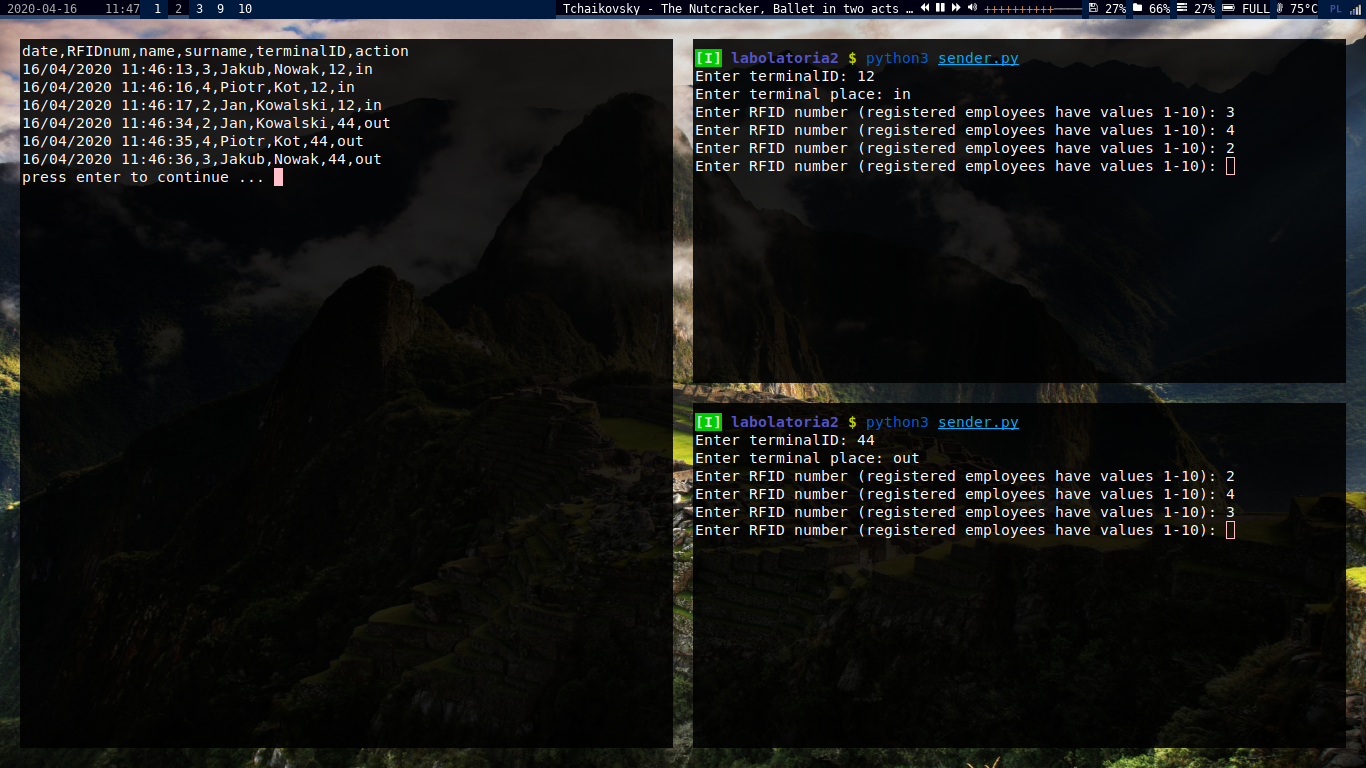
\includegraphics[scale=0.4]{logs}
\end{adjustbox}


\end{document}
